Nyní představíme v~současnosti nejrozšířenější systémy pro \textit{digitální}
řízení modelové železnice. Prozkoumáme zařízení, která tyto standardy
podporují, a~zhodnotíme jejich vlastnosti. Bude vyhodnoceno, jestli zařízení
naplňují požadavky definované v~předchozí kapitole.

\section{Digital Command Control} \label{sec:dcc}

\textit{Digital Command control} (\gls{dcc}) je celosvětově nejrozšířenější
systém pro \textit{digitální}\footnote{\textit{Digitální} znamená, že mezi
jednotlivými prvky řízení proudí digitální data.} řízení modelové železnice
\cite{dcc_systems:web}. K~\gls{dcc} existují alternativy, které však v~Evropě
nejsou rozšířené, proto alternativní systémy nebudeme uvažovat.\footnote{Toto
tvrzení se zakládá na autorových zkušenostech, relevantní studie neexistují.}

\gls{dcc} specifikuje, které komponenty se účastní řízení kolejiště a jak se
tyto komponenty mají chovat – od elektrických standardů (např. doporučený
způsob zapojení vodičů pod kolejištěm) až po komunikační protokoly. \gls{dcc}
je otevřený standard vytvořený organizací \textit{National Model Railroad
Association} (\gls{nmra}), která sdružuje modelářské kluby (a~tedy i~modeláře),
které jsou přímými uživateli systému \gls{dcc}. Systém \gls{dcc} je tedy
navržen modeláři k~naplnění potřeb modelářů.

Jednotlivé prvky systému \gls{dcc} jsou znázorněny v~\ref{fig:dcc-overview}.
Nyní tyto prvky stručně popíšeme.

\begin{figure}[ht!]
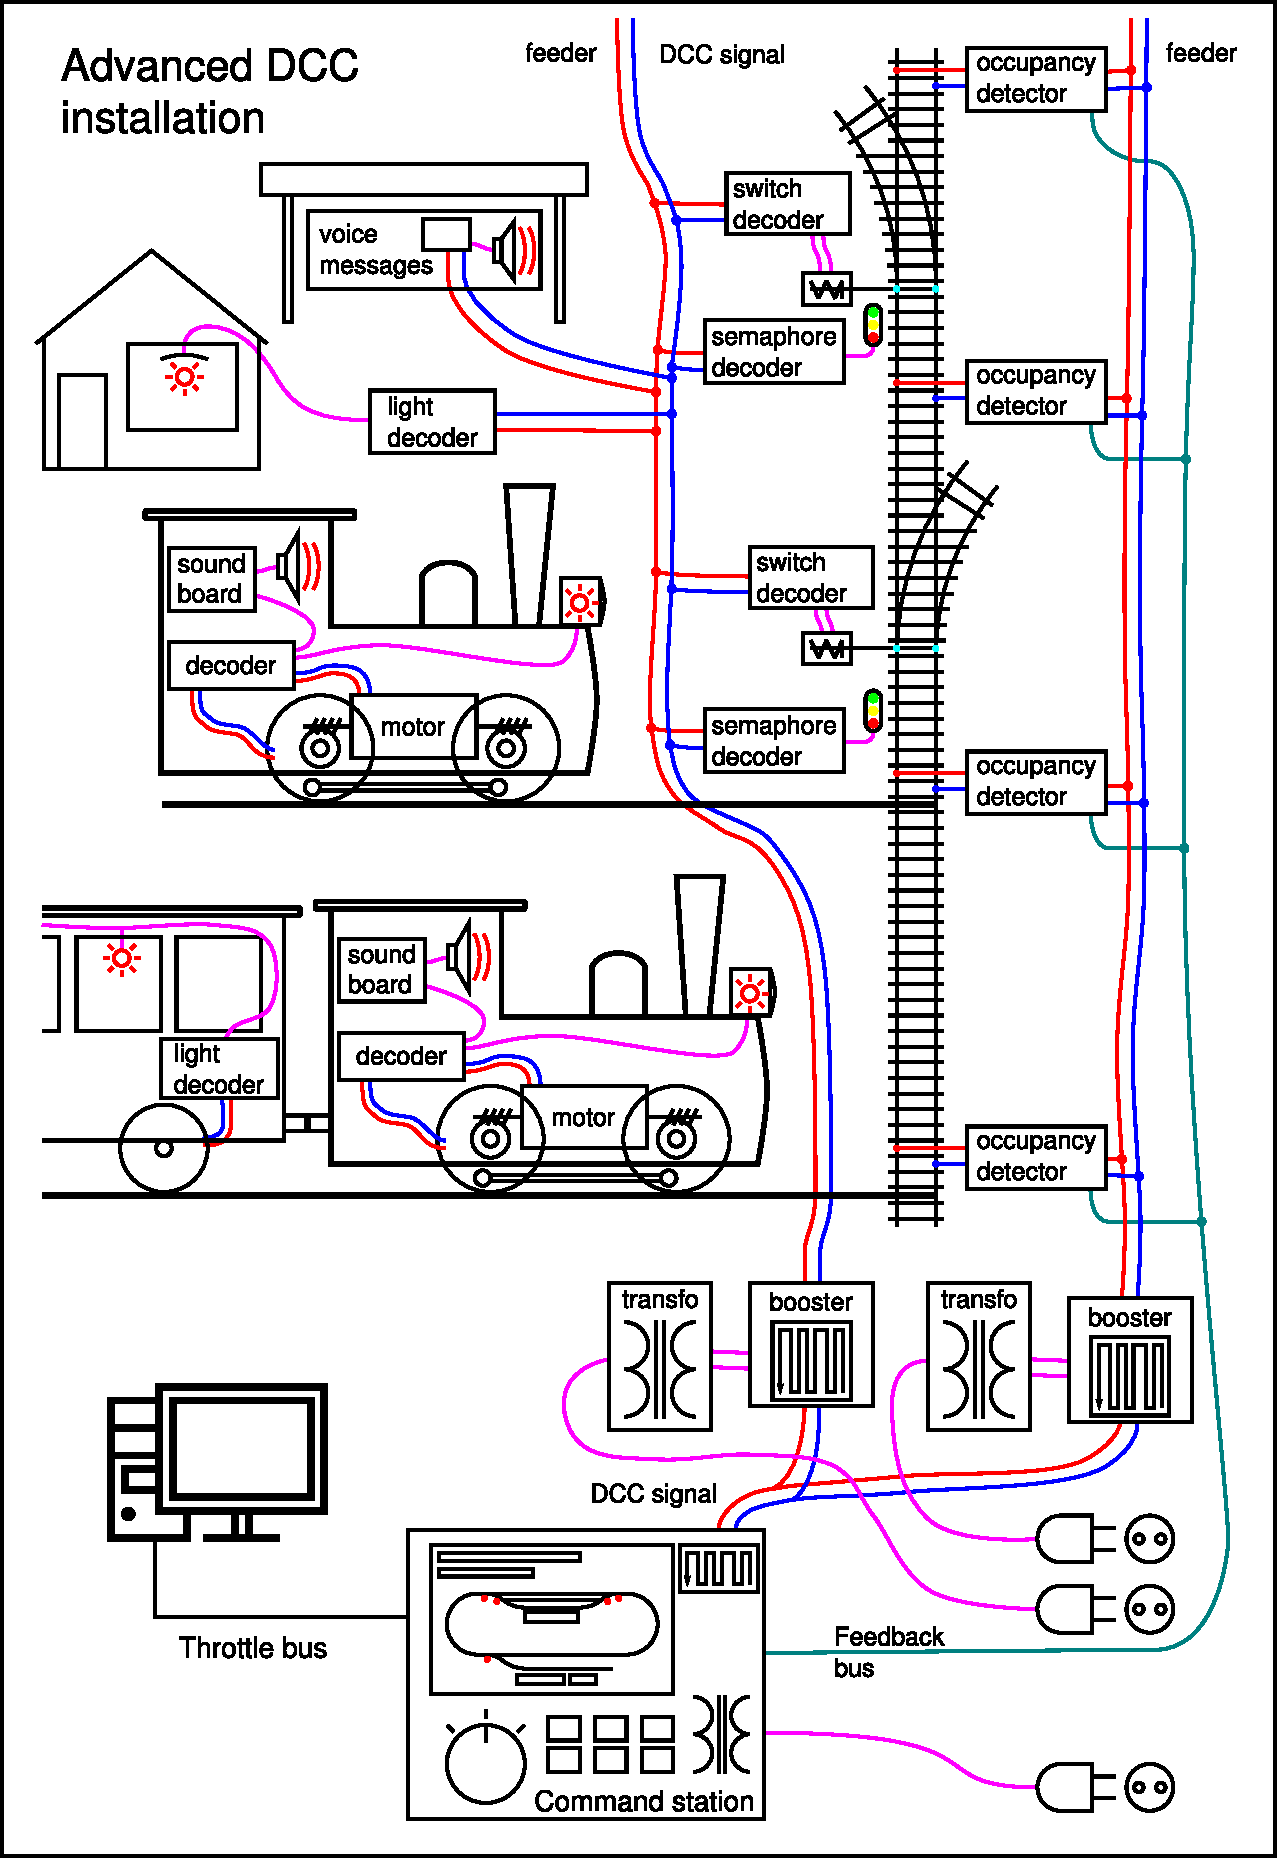
\includegraphics[width=0.95\textwidth]{data/schema_dcc_en.pdf}
\caption{Schéma systému \gls{dcc}. Převzato a upraveno z~\cite{dcc_wikipedia:web}.}
\label{fig:dcc-overview}
\end{figure}

Základní komponentou celého systému je \textit{DCC centrála (Command Station)},
která má 3 hlavní úkoly.

\begin{compactenum}
\item Číst stav \textit{modulů zpětného hlášení} přes \textit{sběrnici zpětného hlášení \\
	(feedback bus)}.
\item Povelovat \textit{dekodéry} (lokomotiv, přestavníků, návěstidel apod.).
\item Obousměrně komunikovat po \textit{sběrnici ovladačů (throttle bus)}.
\end{compactenum}

Řízení dekodérů centrála provádí generováním \textit{DCC signálu} (červený
a~bílý vodič ve schématu \ref{fig:dcc-overview}), do kterého centrála kóduje
operace požadované po dekodérech – např. \uv{dekodére číslo 541, zastav
lokomotivu}, \uv{dekodére číslo 4741, aktivuj čelní světla}.

Ke sběrnici ovladačů jsou připojené buď fyzické ovladače, nebo počítače.
Operátor provozu zadává příkazy, například otočením kolečka ovladače nebo
interakcí s~příslušným software, tyto příkazy jsou přeposlány do centrály,
centrála je dále přeposílá dekodérům, které přímo vykonávají požadované akce.

Na \textit{sběrnici zpětného hlášení} jsou připojeny moduly s~digitálními vstupy,
které jsou namontovány pevně v~kolejišti a~které čtou stav periferií.
Centrála informuje uživatele skrze \textit{sběrnici ovladačů} o~změnách ve
stavech vstupů \textit{modulů zpětného hlášení}. Vstupy modulů zpětného hlášení
jsou připojené například k~signalizacím obsazení \textit{kolejových obvodů},
takže uživatel nebo řídicí SW pozná, že se na koleji nachází nebo nenachází
vlak, dále například koncovým spínačům poloh výhybek, takže řídicí software je
schopen zabezpečit \textit{vlakovou cestu}.

Pro úplnost uvedeme všechny typy vstupů a~výstupů, které se v~\gls{kmz}
používají.

Výstupy:

\begin{compactitem}
\item řízení jízdy lokomotiv,
\item řízení osvětlení lokomotiv a vozů,
\item řízení zvuků lokomotiv,
\item nastavení polohy výhybky, výkolejky,
\item rozpojovač,
\item návěstidlo,
\item přejezd,
\item statické pouliční nebo domovní osvětlení,
\item indikace v~pultu obsluhy.
\end{compactitem}

Vstupy:

\begin{compactitem}
\item indikace obsazení kolejového obvodu,
\item indikace bodového průjezdu vlaku daným místem skrze infračervené čidlo
	(viz \ref{sec:ir}),
\item indikace koncové polohy výhybky,
\item indikace stavu přejezdu,
\item tlačítka v~pultu obsluhy.
\end{compactitem}

Všimněme si klíčové vlastnosti systému: pro řízení dekodérů
a~pro sběr informací z~kolejiště jsou použity 2~různé sběrnice: \textit{dcc
signál} a~\textit{sběrnice zpětného hlášení}. Platí totiž, že signál \gls{dcc}
je pouze jednosměrný. Signál putuje z~\gls{dcc} centrály přes
\textit{zesilovače} a přes koleje do lokomotiv a~vozů, které poveluje.
Existují jen velice omezené prostředky jak dostat data z~lokomotivy zpět do
\gls{dcc} centrály\footnote{Takovému systému říkáme \textit{RailCom}
\cite{railcom:web}.}. Tyto prostředky navíc vznikly až v~pozdějších verzích
normy \gls{dcc}, takže dnes nejsou všeobecně zaužívané \cite{railcom:web}.
Sběrnice \gls{dcc} je tedy prakticky vzato jednosměrná, dokonce bez odpovědí
dekodérů na příkazy

To znamená, že centrála musí DCC příkazy posílat opakovaně, aby zaručila, že je
dekodér skutečně přijme. Může se totiž snadno stát, že lokomotiva zrovna není
schopna přijímat signál – například jede po špinavých kolejích, ze kterých
špatně sbírá. Problém s~přijímáním dat vlivem špatného kontaktu se netýká
\textit{dekodérů příslušenství} (na obrázku \ref{fig:dcc-overview}
\textit{switch decoder} a \textit{semaphore decoder}).  Tyto dekodéry jsou
připojeny pevným kabelem ke kolejím, takže mají nejlepší předpoklady dekódovat
\gls{dcc} signál korektně. Stále však platí, že dekodér neodpoví, že přijal
a~provedl povel. Vykonání povelu mohlo být narušeno čímkoliv od
elektromagnetického rušení signálu až po nepřijetí povelu vlivem chyby ve
firmwaru dekodéru.

Může se zdát, že samotný protokol \gls{dcc} nesplňuje požadavky popsané
v~\ref{subsec:gen_requirements} a~proto jej nemá smysl uvažovat jako nástupce
současného systému \gls{mtb}. Ačkoliv striktně vzato je tento závěr
správný, je nutné si uvědomit širší souvislosti.

Pří řízení provozu na modelovém kolejišti sledujeme mnohé cíle, z~nichž na
prvním místě stojí bezpečnost. Na skutečné železnici je bezpečnost samozřejmě
mnohem důležitější než na železnici modelové. Přesto například materiální škody
vzniklé projetím návěsti zakazující jízdu, vykolejením soupravy, srážky nebo
následného pádu modelu na zem jsou tak markantní, že bezpečnost provozu je
třeba řešit.

Bezpečnost řízení provozu železnice skutečné i~modelové stojí na tom, že
nepustíme vlak do míst, kde by mu hrozila nehoda. K~nehodě může dojít dvěma
způsoby.

\begin{enumerate}
\item \textbf{Vlak stojí a~je nesprávně rozjet do místa, které pro něj není
bezpečné.}

	I~přes to, že dekodéry nepotvrzují přijetí signálu a~provedení akce, této
	situace se jsme schopni vyvarovat. Všechny klíčové komponenty kolejiště,
	které řídí směr pohybu vlaku (výhybky, výkolejky) indikují svůj stav. To
	znamená, že když se nepovede provést například přestavení výhybky vlivem
	nedoručení příslušného \textit{\gls{dcc} paketu}, výhybka se nepřestaví,
	moduly zpětného hlášení správně indikují, že výhybka se nehýbe, řídicí
	software správně vyhodnotí, že nedošlo ke splnění podmínek pro rozjetí
	vlaku a~vlak nerozjede.

	Z~tohoto pohledu tedy nepotvrzování \gls{dcc} příkazů nevede k~nebezpečné
	situaci.

	Jiná situace nastane u~dekodérů, které provádějí akce, aniž by indikovaly
	svůj stav. Takové dekodéry jsou například \textit{dekodéry návěstidel}
	(\textit{semaphore decoder} na obrázku \ref{fig:dcc-overview}). Tyto dekodéry
	však neovlivňují směr jízdy vlaku. Špatná návěst na návěstidle je
	nemodelová, ale ke hmotným ztrátám nedojde.
	\footnote{Jiná situace panuje na skutečné železnici, kde je návěst návěstidla
	důležitým komunikačním prvkem mezi dispečerem a~strojvedoucím. Je nutné,
	aby strojvedoucí viděl správnou návěst, protože nesprávná návěst
	by mu mohla povolit jízdu, přestože se například proti němu blíží vlak. Nebo
	by například mohla povolit jízdu vyšší rychlostí, než jaká je v~daném
	úseku předepsaná a~vlak by pak nemusel stihnout později zabrzdit. Proto se
	na skutečné železnici kontroluje, že světly návěstidel, která mají být
	rozsvícená, skutečně prochází proud.}

\item \textbf{Vlak se nepovede zastavit.}

	Může nastat situace, kdy se vlak blíží k~místu zastavení, řídicí software
	mu správně pošle příkaz k~zastavení, ale lokomotiva přesto nezastaví.
	Například vlivem již popsaného špatného kontaktu lokomotivy s~kolejemi
	a~tudíž neschopnosti řádně dekódovat \gls{dcc} signál. Norma \gls{dcc} totiž
	specifikuje \uv{pokud dekodér nedekóduje signál, zůstává ve stejném stavu}.
	Tedy například lokomotiva se pořád pohybuje vpřed.

	Popsaná situace v~praxi nastává, ale není v~záběru této práce s~ní naložit.
	Tato práce se zaměřuje především na řízení příslušenství a~snímání stavu
	kolejiště, nikoliv na systém řízení jízdy hnacích vozidel.

\end{enumerate}

Závěrem uveďme, že z~dosavadního popisu systému \gls{dcc} plyne, že tento
systém je pro řízení příslušenství vhodný, i~když s~drobnými nedokonalostmi.

\subsection{Sběrnice zpětného hlášení}

V~předchozí kapitole jsme při formulování závěrů vycházeli z~předpokladu, že
jsme schopni bezpečně indikovat stav všech prvků v~kolejišti (pomocí
\textit{sběrnice zpětného hlášení} – \textit{feedback bus} ve schématu
\ref{fig:dcc-overview}). Prozkoumejme spolehlivost této sběrnice.

\gls{nmra} nedefinuje jednotný standard pro \textit{sběrnici zpětného hlášení}
\cite{dcc_specs:web}, různí výrobci používají různé (vlastní) sběrnice
\cite{dcc_feedbacks:web}. Analyzujme nejpoužívanější sběrnice.

\subsubsection{S88}

\textit{S88} je základní sběrnice zpětného hlášení. Její fungování lze v~zásadě
charakterizovat jako \uv{vylepšené posuvné registry} \cite{s88:web}. Jednotlivé
moduly jsou řazeny za sebe, propojují se vždy sousední moduly. První modul je
připojen do \gls{dcc} centrály.

\begin{figure}[ht!]
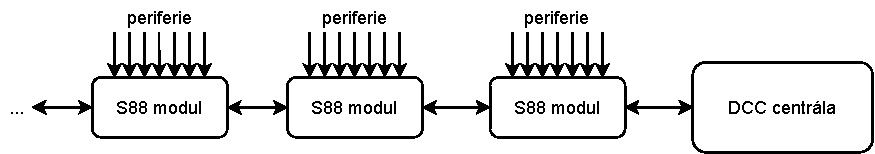
\includegraphics[width=\textwidth]{data/s88.pdf}
\caption{Topologie sběrnice S88.}
\label{fig:s88-topology}
\end{figure}

\textit{S88} je nízkonákladová sběrnice určená pro malá kolejiště. Limitujícím
faktorem je především napájení z~5~V, které není vhodné na delší rozvody,
a~malá odolnost proti rušení \cite{s88:web}.

Jak je patrné z~topologie sběrnice \ref{fig:s88-topology}, při výpadku
(napájení) jednoho modulu jsou ztracena data i~ze všech dalších modulů dále od
centrály. Takové chování je pro profesionální \gls{plc} systém nevhodné.

\subsubsection{RSbus}

\textit{RSbus} je sběrnice firmy \textit{Lenz Elektronik}. Oproti \textit{S88}
je organizována do topologie sběrnice. Jednotlivé moduly jsou napájeny
samostatně, sběrnice je dimenzovaná až na 128 modulů, každý s~8 digitálními
vstupy \cite{rs:web} \cite{rs_lib:web}.

\begin{figure}[ht!]
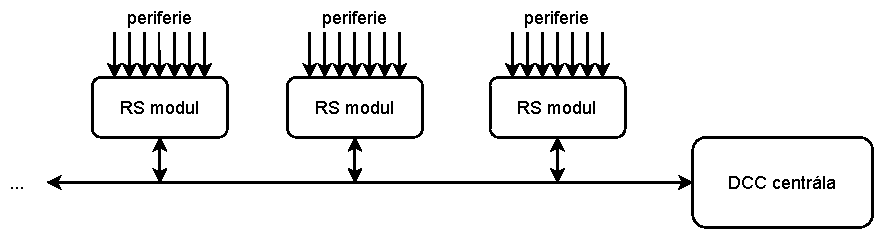
\includegraphics[width=\textwidth]{data/rs.pdf}
\caption{Topologic sběrnice RSbus.}
\label{fig:rs-topology}
\end{figure}

Komunikaci po sběrnici řídí \gls{dcc} centrála – posílá výzvy jednotlivým
modulům a~moduly odpovídají, pokud mají nějaká data k~odeslání. Moduly odesílají
data jen pokud došlo ke změně vstupů, což znamená, že nelze odlišit nefunkční
modul od funkčního modulu se setrvalým stavem vstupů \cite{rs_lib:web}.

Takové chování bohužel nesplňuje požadavky definované
v~\ref{subsec:gen_requirements}. Pokud by například došlo výpadku \textit{RS
modulu} a~následnému obsazení kolejového obvodu, jehož stav tento modul indikuje,
z~pohledu řídicího softwaru by byl kolejový obvod stále volný. Řídicí software
by pak povolil vjezd vlaku na obsazenou kolej, čímž by způsobil srážku.

K~výpadku RS modulu může dojít snadno například ztrátou napájení vlivem chybné
obsluhy, reakce pojistky na přetížení, poruchy apod.

\subsubsection{LocoNET}

Poslední z~analyzovaných sběrnic je \textit{LocoNET}. LocoNET je
proprietární sběrnice společnosti \textit{Digitrax} \cite{loconet:web}, jejíž
plná specifikace není volně dostupná \cite{loconet_license:web}.  Plné použití
této sběrnice podléhá licenčním poplatkům \cite{loconet_license:web}.
Zajímavou vlastností sběrnice je, že slučuje sběrnice \textit{throttle bus}
a~\textit{feedback bus} (viz schéma \ref{fig:dcc-overview}). Řídicí software
v~počítači tak může přímo dotazovat moduly zpětného hlášení a~úplně tak obejít
\gls{dcc} centrálu. Sběrnice LocoNET je navíc obousměrná,
LocoNET moduly jsou vstupně-výstupní, takže počítač může přímo
povelovat periferie \cite{loconet:web}. Viz \ref{fig:loconet-topology}.

\begin{figure}[ht!]
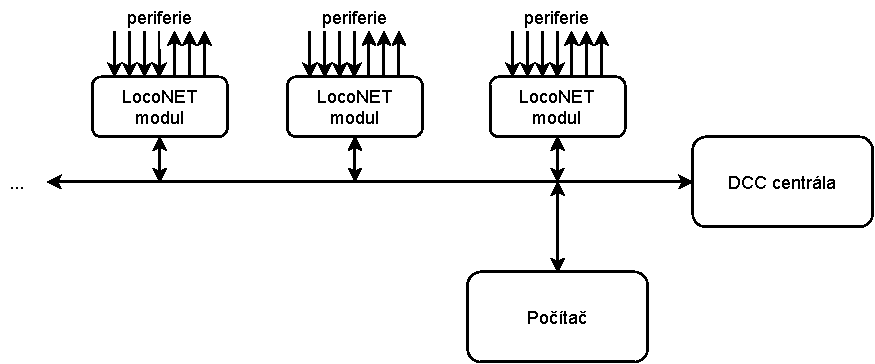
\includegraphics[width=\textwidth]{data/loconet.pdf}
\caption{Topologic sběrnice LocoNET.}
\label{fig:loconet-topology}
\end{figure}

Protokol sběrnice LocoNET umožňuje dotazovat moduly na jejich stav
\cite{loconet-specs}, což umožňuje počítači přímo rozpoznat, které moduly jsou
na sběrnici přítomny, výpadek modulu a~oživení modulu po výpadku.

Sběrnice LocoNET splňuje požadavky na bezpečné řízení periferií
definované v~\ref{subsec:gen_requirements}. Při bližší inspekci však
zjišťujeme, že nasazení této sběrnice by znamenalo nakoupit a~vyměnit cca 100
modulů v~kolejišti. Výměna by navíc musela být rozsáhlejší, LocoNET
moduly přímo nepodporují například generování signálu \textit{\gls{scom}}. Pro
nasazení sběrnice LocoNET by musely být instalovány přídavné moduly
pro řízení návěstidel.

\section{BiDiB}

Zajímavou alternativou k~systému \gls{dcc} je sběrnice \textit{\gls{bidib}}
\footnote{\url{http://bidib.org/}} (\textit{BiDirectional Bus}). \gls{bidib}
je komunitní sběrnice s~otevřeným protokolem, která do velké míry splňuje
všechny požadavky definované v~\ref{subsec:gen_requirements}. Systém \gls{bidib}
lze provozovat na více komunikačních médiích (RS485, Ethernet, sériový port),
návrh systému je podobný návrhu \gls{usb} – na sběrnici je jeden \textit{master},
až 32 \textit{slave} v~každém segmentu, přičemž jedním ze \textit{slave} může
být \textit{hub} vedoucí do dalšího segmentu.

Autoři \gls{bidib} si dali za cíl, podobně jako autor této práce, vytvořit
bezpečný systém pro řízení modelových kolejišť. Systém tak podporuje potvrzování
příkazů, aktualizaci firmwaru modulů apod.

Pro nasazení \gls{bidib} by bylo třeba provést netriviální úpravy
aktuálních modulů kolejiště – \gls{bidib} například definuje standardní
konektory pro propojení modulů. Dále by bylo třeba vyřešit, jak naložit
s~limitem 32 desek v~jednom segmentu sběrnice (protože \gls{mtbbus} je navržen
až pro 255 modulů) a~s~jiným způsobem adresování modulů sběrnice.
\section{Závěr}

V~této kapitole byly popsány základní přístupy k~řízení moderní digitální
modelové železnice. Bylo zkoumáno, jestli komerční produkty splní požadavky
definované v~\ref{subsec:gen_requirements}. Po vyloučení technicky
nezpůsobilých řešení zbyly sběrnice LocoNET (s~poznámkou,
že její nasazení by bylo finančně náročné a~pracné) a \textit{\gls{bidib}}.

Při uvažování sběrnice LocoNET vyvstal problém s~integrací ovládání
návěstidel. Tento problém je obecnějšího rázu – jakékoliv komerční řešení není
schopné nabídnout takovou flexibilitu, jakou bychom v~\gls{kmz} potřebovali.
Je nutné integrovat systém řízení kolejiště se současnými periferiemi, ale
i~s~periferiemi budoucími. Je chtěné mít možnost pružně reagovat na nové
periferie, které se objeví například za 10 let.

Uvažme také aspekt zpětné kompatibility – vlastní systém nám umožní co možná
nejrozumněji zachovat kompatibilitu se stávajícím systémem řízení kolejiště
a~minimalizovat tak finanční náklady a čas nutný pro aktualizaci systému.
Nutnost rozumné zpětné kompatibility tak fakticky vylučuje i~nasazení
\gls{bidib}.

Vnímejme tuto kapitolu tedy především jako přehled technologií, které se
při řízení současné digitální modelové železnice používají. Přistupme k~návrhu,
jak povýšit systém \gls{mtb} výrobou vlastních komponent.
